%%%%%%%%%%%%%%%%%%%%%%%%%%%%%%%%%%%%%%%%%%
% Master Thesis 
% Polina Polunina
% October 2022 
%
% License:
% CC-BY-SA 4.0 -- Creative Commons Attribution-ShareAlike 4.0 International
% https://creativecommons.org/licenses/by-sa/4.0/legalcode
%%%%%%%%%%%%%%%%%%%%%%%%%%%%%%%%%%%%%%%%%%
\section{Introduction}
More than 485 million people have been affected by the \acrshort{covid19} pandemic more than 2.5 years after the first report of \acrshort{sarscov2} in Wuhan, China. During the \acrshort{covid19} pandemic, wastewater surveillance has received extensive public attention as a passive monitoring system that complements clinical and genomic surveillance. The detection and quantification of viral RNA in wastewater samples are already possible through several methods and protocols, and viral RNA concentrations in wastewater have been shown to correlate with reported cases. In the Netherlands, for example, which has had a nationwide wastewater monitoring network for decades, scientists found that fragments of the \acrshort{sarscov2} virus can accurately reflect its level in the community \cite{medema2020}. The correlation was also shown by tracking wastewater samples in Sweden as well as in Switzerland \cite{wang2022,jahn2022}. 

The Galaxy community has put much effort into a continuous analysis of intra-host variation in \acrshort{sarscov2} (https://galaxyproject.org/projects/covid19/) \cite{baker2020,maier2021,mei2021,martin2021}, including the development of workflows, on samples of individuals.
    
The purpose of this thesis is an improvement of existing workflows in Galaxy to support the analysis of wastewater data.

    \subsection{SARS-CoV-2}
        \subsubsection{COVID-19 and pandemic}
        A contagious disease,\acrfull{covid19}, is caused by the \acrfull{sarscov2}. The first reported case occurred in Wuhan, China, in December 2019 \cite{wu2020}, which rapidly evolved into a pandemic.
        
        A public health emergency of international concern was declared by the \acrfull{who} on 30 January 2020 \cite{statement2020}, and a pandemic on 11 March 2020 \cite{who2020,cucinotta2020}. More than 609 million cases have been reported, and more than 6.51 million deaths have been confirmed as of 14 September 2022 \cite{weekly2022}.
        
        There are a range of symptoms associated with \acrshort{covid19}, including fever \cite{islam2021}, cough, headache \cite{islam2021}, fatigue, breathing difficulties, loss of smell  \cite{saniasiaya2021,saniasiaya2021b}, and loss of taste \cite{saniasiaya2021b,agyeman2020}. Virus infection may cause symptoms one to fourteen days after exposure. Infected people develop no noticeable symptoms in at least a third of cases \cite{oran2021}. It has been shown that most people (81\%) with symptoms noticeable enough to qualify as patients develop mild to moderate symptoms, while 14\% develop severe symptoms (dyspnoea, hypoxia, or more than 50\% lung involvement on imaging), and 5\% develop critical symptoms (respiratory failure, shock, or multiorgan dysfunction) \cite{management2020}. There have been reports of damage to organs in people who have suffered a  traumatic brain injury that continues months after they have recovered \cite{cdc2022}.
        
        \acrshort{covid19} spreads when airborne droplets and small particles containing the virus are inhaled. Proximity increases the risk of breathing these. In rare cases, contact with contaminated surfaces can also lead to transmission if splashed or sprayed with contaminated fluids. Even if no symptoms appear, people can spread the virus for up to 20 days \cite{cdc2020b}.

        \subsubsection{SARS-CoV-2 virus}
        Initially, \acrshort{sarscov2} was isolated from three people with pneumonia connected to an acute respiratory illness cluster in Wuhan \cite{risk}. \acrshort{sarscov2} virus particles exhibit all structural features found in related coronaviruses in nature \cite{andersen2020}.
        
        \acrshort{sarscov2} is closely related to the original SARS-CoV \cite{zhu2020}. An animal origin is suspected \cite{zhou2020}. Phylogenetic analysis shows that the Coronavirus clusters with the subgenus Sarbecovirus (lineage B) and two bat-derived strains in the genus Betacoronavirus. 
        
        It is 96\% identical at the whole genome level to other bat coronavirus samples (BatCov RaTG13) \cite{rathore2020}. Several structural proteins are associated with \acrshort{sarscov2}, including membrane glycoproteins (M), envelope proteins (E), nucleocapsid proteins (N), and spike proteins (S). There is about 98\% homology between the M protein of \acrshort{sarscov2} and the M protein of bat SARS-CoV, around 98\% homology with pangolin SARS-CoV, and 90\% homology with the M protein of SARS-CoV; however, the similarity is only 38\% with the M protein of MERS-CoV \cite{thomas2020}.
        
        \subsubsection{SARS-CoV-2 mutations}
        As all viruses mutate, so does \acrshort{sarscov2}. Viruses reproduce (or make copies of themselves) inside host cells and occasionally mutate, e.g., changes appear in the string of 30,000 bases that make up the \acrshort{sarscov2} genome. These mutations may lead to changes in the amino acids that make up a protein, which would alter its structure. A virus that has been mutated may weaken or die out as a result of these changes. In rare cases, mutations can improve the virus's ability to cause disease, spread, or evade host immunity. If the mutations spread with virus replication and invade the virus population, the corresponding virus can become a "variant" of its wild-type (original) by accumulating advantageous mutations, making it a better infector, disease-causing agent, evading the immune system, or spreading within a population \cite{variants}. With over 485 million documented infections during the past two years, and probably many more undocumented, there have been an incredible number of mutation opportunities.  Nevertheless, most of them do not cause global surges and do not pose any more significant threat than existing variants.
        
        In the first year of the Coronavirus pandemic, the virus did not change much. Approximately one or two mutations were picked up by \acrshort{sarscov2} each month. The phylogenetic tree had only one main trunk and a few tiny branches (\cref{fig:intro:corona-timeline}). Pandemic course changed in 2020.
        \begin{figure}[h]
        	\centering
        	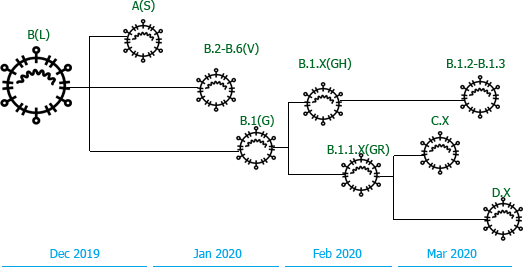
\includegraphics[width=1\textwidth]{figures/intro/corona-timeline.png}
        	\captionof{figure}{Schematic representation of the major evolutionary events that gave rise to \acrshort{sarscov2} variants in sequential order (simplified, cf. \cite{jacob2021}). }
        	\label{fig:intro:corona-timeline}
        \end{figure}
        \subsubsection{SARS-CoV-2 variants}
        From approximately summer of 2020 on, \acrshort{sarscov2}'s family tree grew increasingly complex. The main trunk sprouted branches for a number of variants. Gamma, lambda, and mu variants appeared (although none spread worldwide). The tree's canopy was formed by dozens of branches (\cref{fig:intro:nextstrain}).
        \begin{figure}[h]
        	\centering
        	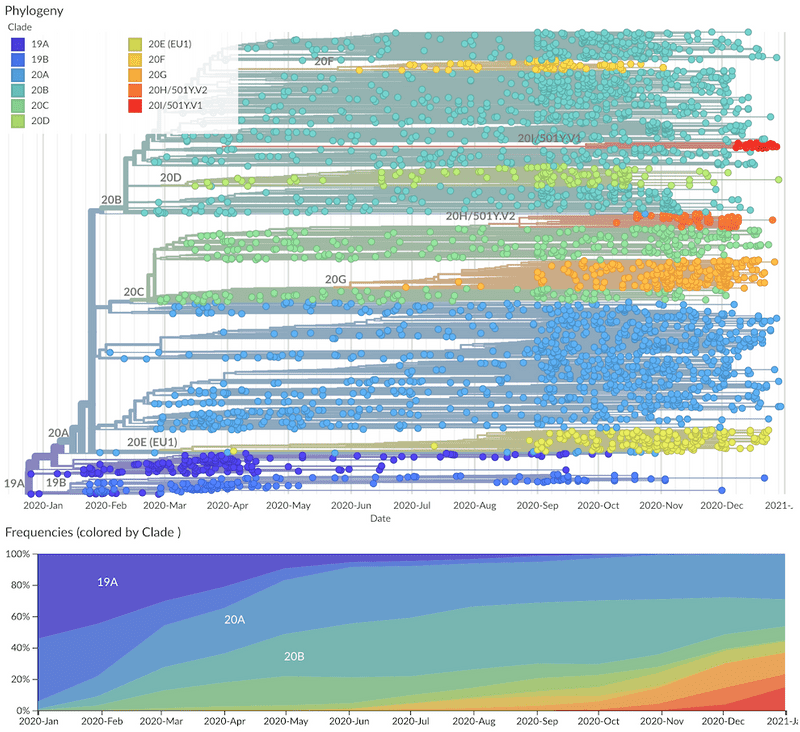
\includegraphics[width=0.7\textwidth]{figures/intro/nextstrain-global.png}
        	\captionof{figure}{\acrshort{sarscov2} phylogenetic tree with a timeline from Nextstrain project labeled by clades (image from \cite{nextstrain2}). }
        	\label{fig:intro:nextstrain}
        \end{figure}
        Researchers track the \acrshort{sarscov2} variants with mutations that are clinically or epidemiologically significant. Detecting variants in a virus usually requires sequencing its complete genome. By sequencing a representative sample of viral specimens in a population, one can determine if new variants are emerging or existing ones are spreading. In particular, variants with the potential or demonstrated ability to be more transmissible, immune evasive, or virulent are closely monitored. These are designated as \acrfull{vois} or \acrfull{vocs}.
        
        On-going pandemic control efforts are challenged by the emergence of \acrshort{sarscov2} variants with greater transmission potential and/or immunity circumvention. In 2020, researchers from South Africa and Great Britain identified two variants of concern \cite{voc2022}: alpha and beta \cite{planas2021}. The virus changed rapidly due to these two variants. According to estimates, each variant had around 20 mutations, compared to a few mutations in previous variants. As a result, they became \acrshort{vocs} instead of \acrshort{vois}.
        \subsubsection{SARS-CoV-2 naming systems}
        Based on genomics experts' rules, several commonly used naming systems \cite{reich} classify the evolving virus forms. The most widely used naming systems are Pango \cite{otoole2021}, which uses the nomenclature system and rules outlined in the publication by Rambaut, A., Holmes, E.C., O’Toole, Á. et al. \cite{rambaut2020} and is maintained by the Pango Network (http://pango.network), and Nextstrain that initially uses ‘year-letter’ naming. Nextstrain nomenclature was first used to monitor and document the Ebola epidemic in West Africa in 2013-2016 and the Zika outbreak in America in 2018. A number of components make up Nextstrain: python scripts maintain a database of sequences and metadata, sourced from public databases such as NCBI (www.ncbi.nlm.nih.gov), GISAID (www.gisaid.org) and ViPR (www.viprbrc.org), as well as GitHub repositories and other genomic data sources. There is a suite of tools available for phylodynamic analysis \cite{volz2013}, including subsampling, alignment, phylogenetic inference, and the reconstruction of discrete trait geographic patterns, including the estimation of the probabilities of transmission \cite{hadfield2018}. As soon as \acrshort{sarscov2} genomes are shared, Nextstrain incorporates them and provides analyses and reports as soon as they are available. Nextstrain \acrshort{sarscov2} naming strategy is in sync with Pango. As an example, Nextstrain clade 22A corresponds to Pango lineage BA.4, 22B to BA.5, and 22C to BA.2.12.1 \cite{nextstrain}. There may be some differences in the classification of viruses across or within lineages or clades, for example, although the major lineages and clades are generally assigned in a similar manner.
        
        Variants were named with different letters and numbers by different groups of scientists, which can be confusing to the general public. As an example, in the beginning of pandemic, many news organizations and others addressing non-scientific audiences had simplified the naming of variants by referring to the countries in which they first appeared, but this could have resulted in stigma, blame, or prejudice. Therefore, The World Health Organization \cite{tracking}, around two years ago, proposed using Greek alphabet letters to label variants of concern and interest in an effort to make their identification easier to pronounce and less stigmatizing. \acrshort{who} has designated five variants as \acrshort{vocs} and given them the Greek letter names Alpha, Beta, Gamma, Delta, and Omicron (\cref{tab:intro:vocs}).
        
        \begin{table}[ht!]
            \centering
            \small
            \begin{tabular}{lllll}
            \textbf{\acrshort{who}} & \textbf{Pango}               & \textbf{GISAID}    & \textbf{Nextstrain}   & \textbf{Earliest date} \\ \hline
            Alpha                   & B.1.1.7                      & GRY                & 20I (V1)              & September 2020 \\
            Beta                    & B.1.351                      & GH/501Y.V2         & 20H (V2)              & May 2020 \\
            Gamma                   & P.1                          & GR/501Y.V3         & 20J (V3)              & November 2020 \\
            Delta                   & B.1.617.2 and AY Sublineages & G/478K.V1          & 21A,21I,21J           & October 2020 \\
            Omicron                 & B.1.1.529 and BA Sublineages & GR/484A            & 21K,21L,21M           & November 2010\\ \hline
            \end{tabular}
            \caption{Designated \acrlong{vocs} named by different naming systems} \label{tab:intro:vocs}
        \end{table}
       
        \subsubsection{SARS-CoV-2 tracking projects}
        \acrshort{sarscov2} variants began to be tracked from the beginning of the \acrshort{covid19} pandemic in order to observe global trends of \acrfull{vocs} (\cref{fig:intro:voc-growth}).
        \begin{figure}[h]
        	\centering
        	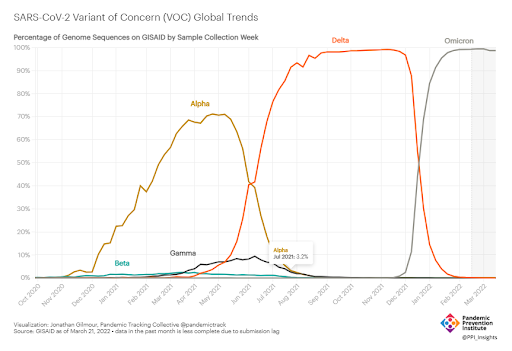
\includegraphics[width=0.7\textwidth]{figures/intro/voc-growth.png}
        	\captionof{figure}{Chart of global \acrshort{sarscov2} \acrshort{voc} growth from 4 October, 2020, to 21 March, 2022 (image from \cite{variants}). }
        	\label{fig:intro:voc-growth}
        \end{figure}
        
        The Delta (B.1.617.2) variant was dominant worldwide between June and December 2021, it has 13 mutations and over 200 known sublineages. Compared to the original virus sequenced in January 2020, the Omicron variant was found to have 50 mutations, when sequenced for the first time in November 2021, and has more than 300 sublineages by now, according to Pango Lineages database https://cov-lineages.org/. In the middle of 2020, once Omicron's lineage diverged, it became phylogenetically distinct from other known \acrshort{vocs} or \acrshort{vois} \cite{otoole2021}. However, the Omicron variant reached its peak worldwide in January 2022 and continues to be prevalent compared to other variants of concern. 
        
        In the course of the \acrshort{covid19} pandemic, many laboratories have developed genomic epidemiology data infrastructures. By January 2022, there were nearly 4000 unique labs submitting data to the GISAID EpiCoV database. A consortium called COG-UK \cite{cogconsortium} is one of the well-known \acrshort{sarscov2} tracking projects. Their research built on the availability of \acrshort{sarscov2} genomes generated throughout the pandemic and spanned across variants, data linkage, and quality. Moreover, there are other complementary projects focused on the emergence of \acrshort{sarscov2} variants. At the beginning of the \acrshort{covid19} pandemic, a problem with available data to analyze occurred \cite{baker2020}. In this regard, COG-UK is the \acrshort{sarscov2} data tracking project that reflected quickly to that and was one of the first that shared data for publicity. Another example of a tracking project that is focused on \acrshort{sarscov2} sequencing is the Swiss \acrshort{sarscov2} Sequencing Consortium (S3C) \cite{chen2022,swiss}.
        
        Currently, large amounts of sequencing data have become increasingly available and must be constantly analyzed. As a result of these data, one can monitor the emergence and spread of new variants, as well as understand the viral evolution dynamics.

    
    \subsection{Surveillance of SARS-CoV-2}
    In order to respond effectively to \acrshort{sarscov2}, global surveillance is essential for determining which variants require closer monitoring as possible threats to public health. Health professionals and policymakers should have up-to-date information about viral populations present in communities, particularly as new \acrshort{sarscov2} variants emerge that alter viral fitness and/or pathogenesis.
    
    A variety of surveillance techniques are available for \acrshort{sarscov2}. Clinical testing was the most potent and widespread method at the beginning of the pandemic. Different types of clinical testing are possible now. For example, diagnostic testing is one of the clinical testing types and is intended to identify current infections in individuals who have symptoms consonant with \acrshort{covid19} and/or have recently been exposed to \acrshort{sarscov2}. The other type of clinical testing - screening testing - is used for identifying asymptomatic individuals with \acrshort{covid19} cases who don't have known, suspected, or reported exposure to \acrshort{sarscov2} \cite{cdc2020c}.
    
    In addition to clinical testing, public health surveillance entails the systematic collection, analysis, and interpretation of health-related data that are essential for planning, implementing, and evaluating public health practices. An important purpose of surveillance testing in public health is to monitor outbreaks of disease at the community and population level, as well as to characterize disease incidence and prevalence. De-identified specimens are used for surveillance testing, so results are not linked to individuals. To determine if the prevalence of viruses is increasing or decreasing in a particular population, a certain percentage of the population may be sampled for public health surveillance testing \cite{cdc2020c}.
    
    A particular type of public health surveillance testing is the surveillance of wastewater by high-throughput sequencing. By monitoring wastewater in a community, one can get a better understanding of the types and amounts of viruses and bacteria that are spreading. The virus RNA in stools of people with current or recent \acrshort{sarscov2} infections is detectable in wastewater samples even if they aren't symptomatic. The cost-effectiveness of wastewater sampling comes from the fact that a single sample can reveal information about an entire building, town, or county. It has been suggested that wastewater surveillance could also be used to detect emerging viral variants in an area as they emerge, in addition to tracking \acrshort{sarscov2} transmission levels.

        \subsubsection{Surveillance from “clinical” data}
        In this section, I will generally discuss the process of lineage identification from isolates with a focus on clinical data surveillance techniques. Starting with sequencing platforms used, I will move to sequencing approaches (e.g. ampliconic-based, metatranscriptomics, etc.) that are used for the extraction of samples with \acrshort{sarscov2}. It should be said that I will mostly focus on metatranscriptomics and ampliconic-based approaches because these two library preparation techniques are used more often for \acrshort{sarscov2} datasets, and in this thesis, I will process and analyze datasets extracted with the help of these two methods. After that, I will explain the bioinformatics steps of data processing, followed by existing solutions suggested by Galaxy Project for clinical \acrshort{sarscov2} data. \\
        
        \textbf{Sequencing platforms} \\
        
        The majority of \acrshort{sarscov2} sequence data is generated using two sequencing platforms: \acrfull{illumina} and \acrfull{ont}. \\
        
        \textbf{\acrshort{illumina} sequencing} \\
        
        \acrshort{illumina} sequencing, the second-generation sequencing, detects the sequence of RNA by using reversible dye terminators technology. Solexa company, now part of Illumina company, invented the reversible dye terminators technology and engineered polymerases that are used in this sequencing method.
        
        \acrshort{illumina} sequencing begins with the cleavage of the sample into short sections.  A short read or fragment of 100-150bp is created at the start of the \acrshort{illumina} sequencing process. The fragments are then ligated to generic adaptors and annealed to slides. Each fragment is amplified by \acrfull{pcr}. By doing this, the same fragment appears in many copies. Sequencing slides contain fluorescently labeled nucleotides, RNA polymerase, and terminator molecules. As a result of the terminator, only one base is added at a time. It allows the next base to be added to the site after each cycle terminator is removed. In each cycle, the computer detects the base added by relying on fluorescent signals \cite{difference2021}. \\
        
        \textbf{\acrlong{ont} sequencing} \\
        
        Nanopore sequencing is the third-generation sequencing technique that detects the RNA sequence by using a protein nanopore. Nanopore sequencing involves RNA passing through a nanopore and changing its current. There is a relationship between the size, shape, and length of the RNA sequence and how a current changes. In order to obtain the specific RNA sequence, the resultant signal needs to be decoded. There is no need to modify nucleotides, and the method works in real-time.
        
        A number of nanopore sequencing devices are manufactured by \acrlong{ont}. Flow cells are a common feature of \acrshort{ont} sequencing devices. An electro-resistant membrane surrounds a number of tiny nanopores in this flow cell. Each nanopore corresponds to its own electrode. An electrode connects to a sensor chip and a channel. A nanopore's electric current is measured by this electrode. As molecules pass through nanopores, their current is changed or disrupted. A characteristic squiggle results from this disruption. Squiggles are decoded in real-time to determine RNA sequences \cite{difference2021}. \\
        
        \textbf{Comparison of \acrshort{illumina} and \acrshort{ont}} \\
        Nanopore sequencing uses a nanopore to detect the RNA sequence, while \acrshort{illumina} sequencing technique uses reversible dye terminators technology to detect the sequence of RNA. Both techniques have markedly high accuracy. More precisely, \acrshort{ont} sequencing has 92-97\% accuracy, while \acrshort{illumina} sequencing has 99\% accuracy. The following \cref{tab:intro:ont-vs-illumina} lists the differences between \acrshort{ont} and \acrshort{illumina} sequencing.
        
        \begin{table}[ht!]
            \centering
            \small
            \begin{tblr}{l|ll}
                                        & \textbf{\acrshort{ont}}                   & \textbf{\acrshort{illumina}} \\       \hline
            \textbf{Generation}         & third-gen                                 & second-gen \\                         \hline[dashed]
            \textbf{Founded by}         & Prof. David Deamer                        & Prof. Shankar Balasubramanian \\
                                        &                                           & and Sir David Klenerman \\            \hline[dashed]
            \textbf{Accuracy}           & 92-97\%                                   & 99\% \\                               \hline[dashed]
            \textbf{Long/short read}    & long reads                                & short reads \\                        
            \textbf{sequencing}         &                                           &  \\                                   \hline[dashed]           
            \textbf{Read length}        & 2,272,580 bp                              & 75-300 bp \\                          \hline[dashed]
            \textbf{Time taken}         & Real time                                 & 4 to 56 h \\                          \hline[dashed]
            \textbf{Cost}               & \$7-100                                   & \$5-150 \\                            \hline[dashed]
            \textbf{Advantages}         & longest individual reads                  & potential for high sequence yield \\  \hline[dashed]
            \textbf{Disadvantages}      & lower throughput than other machines      & expensive \\                          \hline
            \end{tblr}
            \caption{Comparison of \acrfull{illumina} and \acrfull{ont} sequencing} \label{tab:intro:ont-vs-illumina}
        \end{table}

        \textbf{Sequencing approaches} \\
        
        In addition to choosing a sequencing platform, choosing the most appropriate sequencing strategy depends on the final objectives and the type of biological sample. Currently, four different concepts have been applied: 1) shotgun metatranscriptomics, 2) hybrid capture enrichment, 3) amplicon sequencing, and 4) direct RNA sequencing. To make a comparison between sequencing strategies, \cref{tab:intro:seq-approaches} shows the main characteristics.
        
        \begin{table}[ht!]
            \centering
            \small
            \begin{tblr}{l|llll}
                                     & \textbf{Shotgun}             & \textbf{Amplicon-}    & \textbf{Hybrid}           & \textbf{Direct RNA} \\ 
                                     & \textbf{metatranscriptomics} & \textbf{based}        & \textbf{capture-}         & \textbf{sequencing} \\ 
                                     &                              &                       & \textbf{enrichment}       &  \\ \hline
            Goals                   & \acrshort{sarscov2},             &\acrshort{sarscov2}             & \acrshort{sarscov2}               & \acrshort{sarscov2}, \\
                                    & host microbiota,                  & genome                        & genome                            & host \\
                                    & host response                     &                               &                                   & transcriptome, \\
                                    &  to infection                     &                               &                                   &  epitranscriptome\\ \hline[dashed]
            Co-infection            &  Yes                              &  No                           &    No/yes (depending              & \\
            detection               &                                   &                               & on gene panel)                    & Yes \\ \hline[dashed]
            Min number of reads     & 20–50 M                           & 5–20 M                        & 5–20 M                            & 0.5 M \\ \hline[dashed]
            Genome Coverage         & 	\begin{math}\geq 99\% \end{math}                 & 	\begin{math}\geq 95-99\% \end{math}          & 	\begin{math}\geq 95-99\% \end{math}              & 	\begin{math}\geq 99\% \end{math} \\ \hline[dashed]
            Accuracy in \acrshort{snv}  & High                          & High                          & Moderate                          & Moderate \\
            identification          &                                   &                               &                                   & \\  \hline[dashed]
            Sample viral load       & <24–28                            & \begin{math}\geq 24-28 \end{math}     & \begin{math}\geq 24-28 \end{math}         & <24–28 \\
            (Ct) requested          &                                   &                               &                                   & \\ 
            (ref Xiao)              &                                   &                               &                                   & \\  \hline[dashed]
            Sample RNA input        & 10–200                            &      	1–50                    &      10–50                        & \begin{math}\geq 1000 \end{math}\\ 
            (ng)                    &                                   &                               &                                   & \\  \hline[dashed]
            Sample type             & Patient                           &      Patient                  &     Patient                       & Viral  \\  
                                    &   specimens                       &      specimens,               &     specimens,                    & cell \\  
                                    &                                   &      environmental            &     environmental                 & cultures \\  
                                    &                                   &       samples                 &      samples                      & \\  \hline[dashed]
            Cost                    &  High                             &       Low                     &       Moderate                    & High \\ \hline[dashed]
            \acrshort{ngs}          & High- or                          &        Mid-                   &    Mid- or                        & \acrshort{ont} \\ 
            platforms               &  ultra high-                      &         throughput            &      high-                        & \\  
                                    &  throughput                       &         platforms             &      throughput                   & \\  
                                    &   platforms                       &                               &      platforms                    & \\  \hline
            \end{tblr}
            \caption{Comparison of \acrshort{sarscov2} sequencing approaches} \label{tab:intro:seq-approaches}
        \end{table}
        
        Most of \acrshort{sarscov2} sequence data is generated using two established library preparation strategies: ampliconic-based sequencing approach and metatranscriptomics sequencing approach. These two approaches will be discussed in more detail in the following two sections. \\

        \textbf{Metatranscriptomics sequencing approach} \\
        
        In this method, RNA fragmentation is followed by first- and second-strand cDNA synthesis, and then library preparation is carried out based on the high-throughput sequencing techniques of choice \cite{chiara2020}. Metatranscriptomic sequencing is able to detect all types of pathogens, which is beneficial. A complete or nearly complete viral genome can be sequenced and reconstructed from available SARS-CoV-2 sequence data that have enough viral loads. However, most preparation protocols involve multiple costly and complicated steps, which inevitably compromises the effectiveness of sequencing of time-sensitive SARS-CoV-2 samples and in identifying other pathogens \cite{meng2021}.
        
        \Cref{fig:intro:metatr-process} shows a simplified schematic representation of the common wet-lab process for SARS-CoV-2 RNA extraction by metatranscriptomics sequencing approach.
        
        \begin{figure}[h]
        	\centering
            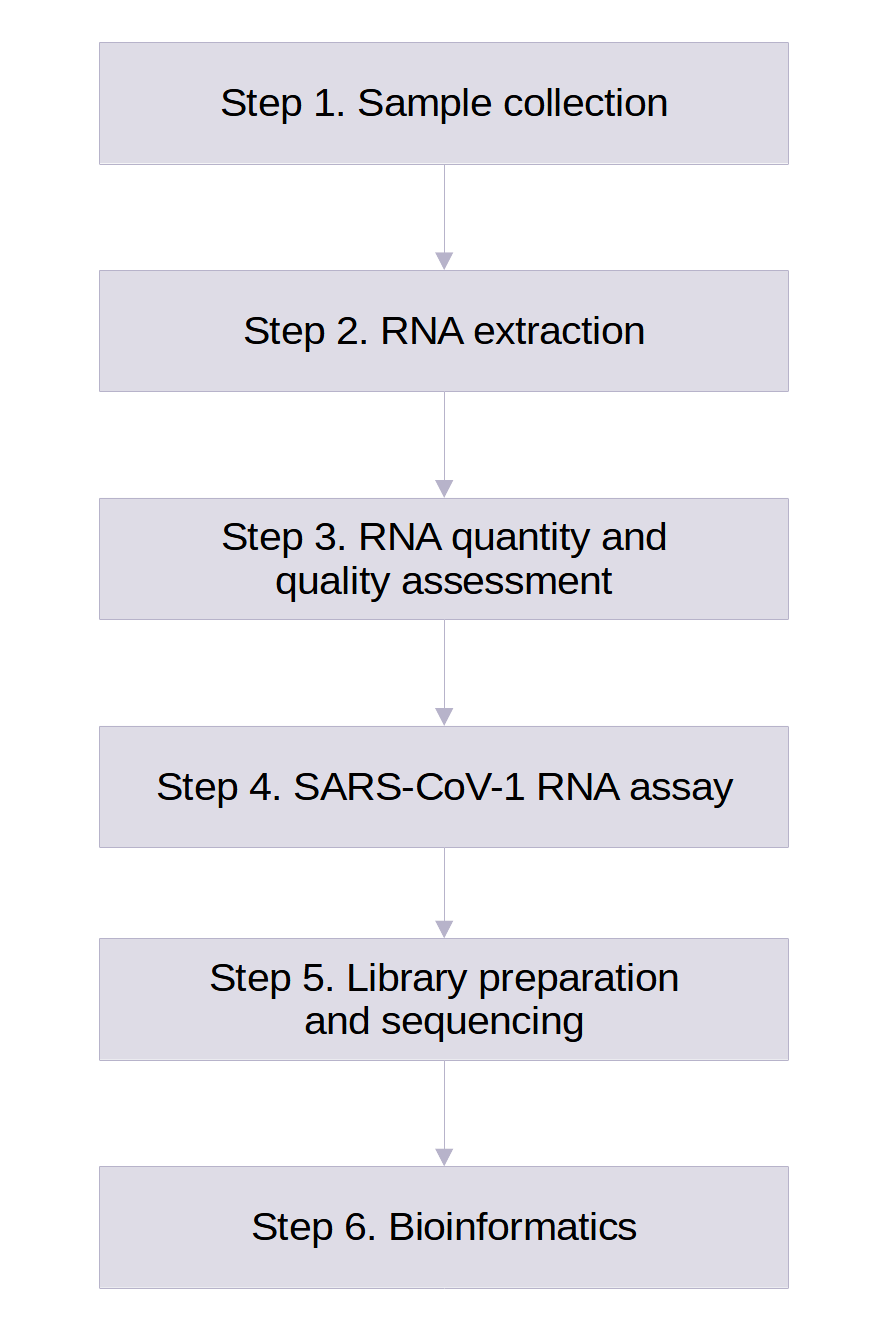
\includegraphics[width=0.5\textwidth]{figures/intro/metatranscriptomics-process.png}
            \captionof{figure}{Schematic representation of the common wet-lab process for \acrshort{sarscov2} RNA extraction by metatranscriptomics sequencing approach (simplified, cf. \cite{chiara2020}). }
            \label{fig:intro:metatr-process}
        \end{figure}
        
        In short, the typical workflow of shotgun metatranscriptomics involves breaking RNA into fragments, synthesizing cDNA from the first and second strands, and preparing a library using the chosen next-generation sequencing technology.\\

        \textbf{Ampliconic sequencing approach (ARTIC protocol)} \\
        
        Amplicon sequencing is a highly targeted approach for analyzing genetic variation in specific genomic regions. This sequencing method provides information about the targeted sequence. If the targeted sequences are rich in lineage-defining polymorphisms, polymorphisms in the target can be easily linked and lead to easier lineage identification. Deep sequencing of polymerase chain reaction (PCR) products (amplicons) facilitates the efficient identification and characterization of variants. Using oligonucleotide probes, regions of interest are targeted and captured. The amplicon sequencing approach is particularly useful for metagenomics samples of diverse origins.

        The use of amplicon sequencing allows researchers to limit the type and number of sequences that can be analyzed. Despite its high specificity, this method requires significant prior knowledge of the sequence that will be 'targeted’. SARS-CoV-2 genome sequencing by amplicon-based methods employs a workflow in which first-strand cDNA is synthesized, followed by multiplex PCR. Pools of amplicons, covering the entirety or discrete portions of the viral genome, are produced. For SARS-CoV-2, several different multiplex PCR designs have been proposed, varying in the number and size of amplicons \cite{chiara2020}.
        
        The ARTIC Network's amplicon-based protocol is one of the most widely used SARS-CoV-2 sequencing protocols \cite{lambisia2022,rd2020,rd2022,quick2020} The protocol relies on direct amplification of the virus using tiled, multiplexed primers. This approach has been proven to have high sensitivity and work directly from clinical samples.
        
        The amplicon sequencing approach has several advantages. Through a highly targeted approach, researchers can discover, validate, and screen genetic variants efficiently. High coverage can be achieved by multiplexing hundreds to thousands of amplicons per reaction. The amplicon sequencing method delivers highly targeted resequencing even in difficult-to-sequence areas. It allows for reducing the cost and time of sequencing compared to other approaches, such as whole-genome shotgun sequencing. But most importantly, it reduces the amount of starting material required. For instance, it is impossible to do non-ampliconic sequencing from nasal swabs, so an ampliconic-based approach should be applied in this case.
        
        In spite of the fact that amplicon sequencing is theoretically convenient and inexpensive, it has some limitations that should be taken into account. As it is stated in a quick guide to tiling amplicon sequencing and downstream bioinformatics analysis \cite{grubaugh2019,loman}, several challenges may arise during the sequencing and analysis process, including contamination, bar-coding issues, and primer binding issues. As a result of the significantly high sensitivity, even a small amount of contaminating templates (such as amplicons from previous work) can lead to the amplification of sequences not present in the sample. The presence of sequences from other samples can confuse the analysis since there is a small rate of barcode "cross-over." Because PCR relies on synthetic primers, amplicons contain synthetic sequences in their primer binding sites. This is a problem that must be accounted for if the primer sequence contains mismatches compared to the template. Additionally, amplification across the genome can be biased by differences in primer efficiency or possible variations in primer annealing regions. For example, specific genomic regions \cite{itokawa2020} may have less coverage, and/or 3' and 5' untranslated regions may be missed altogether, resulting in incomplete assembly. Due to the fact that the primers are designed using the reference SARS-CoV-2 genome sequence, this approach may not be capable of identifying long structural variants, and high levels of genomic divergence can pose systematic limitations.
        
        A recent study suggests that, although the amplicon-based approach is highly reliable for reconstructing a viral population's most prevalent genome variant, it has a highly biased representation of minor allele frequencies compared to metatranscriptomics experiments conducted on the same samples \cite{xia2020}.\\

        \textbf{Data processing with bioinformatics methods} \\
        
        For the next step after sequencing, bioinformatics analysis should be executed. Tools can differ from one pipeline to another. But the main steps, in general, are more or less the same. After getting raw data reads, they have to be processed with different steps. First, quality control, then primer trimming if they were used, and adapter trimming. After that, the decontamination step can be included to remove reads from the human genome. The next crucial step is mapping with reference SARS-CoV-2 sequence. Some steps in pipelines can be done, such as removing duplicates or remapping, but they are not always included. After mapping, variant calling should be run, followed by mutation annotation. 

        There is a number of publications describing different combinations of bioinformatics steps and tools used to process and analyze raw data \cite{baker2020} and ranging from transparent to opaque \cite{holshue2020}. Analytical transparency is crucial for such cases. Now, many organizations provide transparency to data processing and analyzing approaches. For example, the COG-UK datasets, protocols, methods, and techniques for collecting and preparing SARS-CoV-2 virus samples for sequencing, as well as short-read and long-read sequencing, are all publicly available \cite{quick2020}.
        
        Nevertheless, transparent and freely available infrastructure for such analysis is not present everywhere. It is often the case that infectious disease outbreaks occur in remote areas without adequate infrastructure or in political situations that make unbiased interpretation of results impossible. In response, there is a need for free, open, and robust analytical approaches accessible to everyone worldwide for data analysis, interpretation, and sharing. \\

        \textbf{Galaxy effort to surveillance data processing} \\
        
        In order to address global health emergencies in an accessible and transparent manner, there is a need for scientific computing infrastructure to help bridge these gaps. Data and data analysis transparency were the primary focus of the Galaxy effort.

        Through its graphical web interface, Galaxy allows users to use tools from a variety of domains for FAIR \cite{wilkinson2016} data analysis; run code in interactive environments (RStudio, Jupyter, etc.) along with other tools or workflows; manage data by sharing and publishing results, workflows, and visualizations; ensure reproducibility by capturing information that allows data analysis to be repeated and understood \cite{baker2020}.
        
        Galaxy offers powerful public computational infrastructures designed specifically for research purposes in the United States, the European Union, and Australia. In the United States, there is the XSEDE \cite{towns2014} consortium; in the European Union, there is the deNBI \cite{elixirde} and ELIXIR \cite{elixir2,elixir} consortiums; and in Australia, there is the Nectar Cloud consortium. Due to their global accessibility, support for diverse configuration schemes (from traditional computational clusters to fully virtualized cloud-like setups), and ability to provide cutting-edge hardware, large-scale public computing resources are well suited to tackling the bioinformatics challenges of the current pandemic. 
        
        In combination with open-source software tools, this public computational infrastructure offers a complete solution to the SARS-CoV-2 data analytics challenge. Galaxy provides a glue to bind these into a unified analytics platform that manages users, allocates storage, and pairs analysis tools with computational resources fluidly. The platform provides both a graphical user interface and programmatic access in order to accommodate researchers with different degrees of computational expertise. \\

        \textbf{Four SARS-CoV-2 analysis workflows} \\
        
        Based on Galaxy there were four workflows developed aimed at SARS-CoV-2 clinical data analysis. A special webpage was created to track Galaxy efforts on SARS-CoV-2 analysis, workflows, data, and documentation \cite{galaxyproject}. There is a collection of Galaxy workflows for detecting and interpreting sequence variants in SARS-CoV-2. These workflows can be accessed immediately and freely in three global Galaxy instances: in the United States, the European Union, and Australia. 
        
        When creating workflows for SARS-CoV-2 analysis, Maier et al. \cite{maier2021b} took several goals into account. They aimed to provide continuous analysis of within-host sequence variants in high-quality public read-level databases. The other goal was to provide maintenance of curated workflows for the analysis of SARS-CoV-2 sequence data and free powerful infrastructure to execute them, such as Galaxy infrastructure. They developed a continuously updated analysis page and dashboard summarizing the latest insights from the variant. Last but not least focus was to provide access to all results in raw and aggregated form for immediate use.
        
        As suggested by Maier and colleagues, SARS-CoV-2 clinical data analysis is organized into two stages of analysis (\cref{fig:intro:galaxy-effort}). It is computationally intensive at Stage 1, which takes raw sequencing data as input and produces intermediate summaries such as allelic variants and annotations in mutation annotation format (MAF files) and variant calling format (VCF files). Basically, at Stage 1, depending on library preparation and data sequencing method, the appropriate workflow is taken. Thereby, for datasets prepared by using ARTIC amplicon-based protocol, two workflows are available: for datasets sequenced with Oxford Nanopore Technology (ONT) and Illumina-based technology (Illumina). As for datasets prepared with metatranscriptomic protocol, there are two workflows available for Illumina-based sequencing technology. The difference is in the types of reads obtained. One workflow works with paired-end reads, while another one works with single-end reads.
        
        Interpreting and visualizing the Stage 1 outputs are the focus of Stage 2. Additional reporting workflow is developed to analyze outputs of Stage 1, which generates tabular and JSON files. These files serve as input for analysis based on two software systems, Jupyter, and ObservableHQ, for visualizing results.
        
        \begin{figure}[h]
        	\centering
            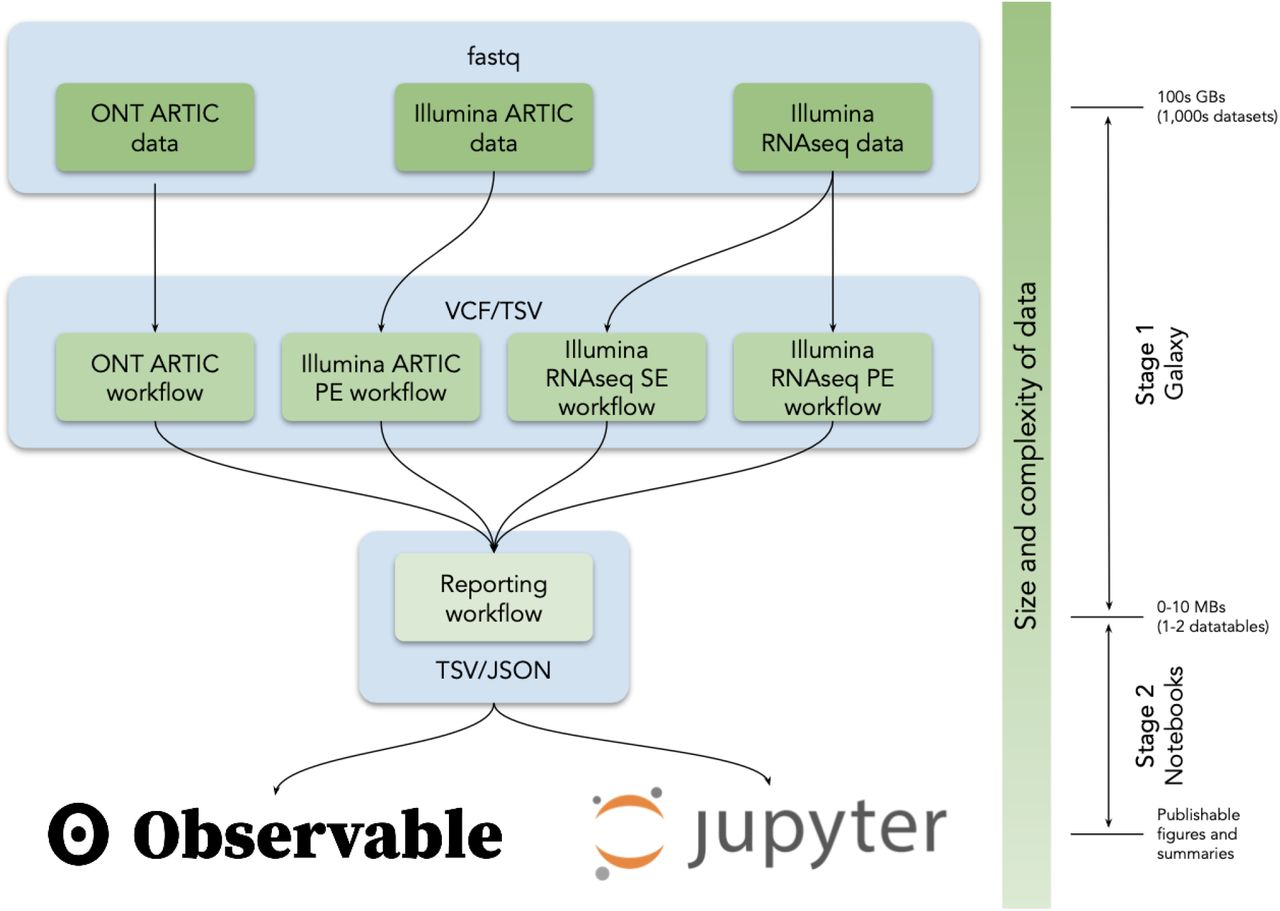
\includegraphics[width=0.7\textwidth]{figures/intro/galaxy-analysis.jpg}
            \captionof{figure}{Analysis flow in the analysis system suggested by GalaxyProject (image from \cite{maier2021b}). }
            \label{fig:intro:galaxy-effort}
        \end{figure}
        
        The choice of bioinformatics tools for these four workflows is made based on the method of sequencing and the type of data obtained by the method. For paired-end reads, the BWA-MEM \cite{li2013,burrows} mapper is used to map to the SARS-CoV-2 sequence. Bowtie2 \cite{ultrafast,langmead2012} mapper is used for single-end read datasets sequenced with Illumina method, whereas minimap2 \cite{burrows,li2018} mapper is most appropriate for datasets sequenced by Oxford Nanopore since Oxford Nanopore sequencer generates very long reads with many errors. As for variant caller, LoFreq is used in all four workflows since it is known as a more ultra-sensitive variant caller for uncovering cell-population heterogeneity \cite{lofreq}.\\

        \textbf{Bots for automated SARS-CoV-2 surveillance } \\
        
        Additionally, Galaxy team has developed bots to assist in SARS-CoV-2 surveillance \cite{bots2022}. Bots for SARS-CoV-2 genome surveillance provide a viable tool for automating the analysis of a large number of SARS-CoV-2 sequences regularly. A bot is a set of automation scripts that can be integrated into any scheduling system with a daily throughput of around 1000 samples on a Galaxy instance. Galaxy bots allow you to upload newly available data, start a variation analysis workflow, and follow up with downstream workflows for consensus building and reporting once the variation analysis is complete. It is possible to use bots for SARS-CoV-2 surveillance to track National Genome Surveillance projects, such as COG-UK, and reanalyze their data as it becomes available. These scripts are a decent automated sequence data analysis pipeline that works with two Galaxy SARS-CoV-2 surveillance workflows for datasets extracted with ARTIC protocol. 
        
        Galaxy workflows developed for SARS-CoV-2 clinical surveillance have shown adequate results. There are, however, some limitations. Currently, Galaxy workflows do not focus on wastewater surveillance. Thus, Galaxy workflows can be improved and repurposed to improve SARS-CoV-2 wastewater surveillance. The current thesis attempts to focus on it.

        \subsubsection{History of wastewater surveillance}
        
        In this section, I will present the introduction to wastewater surveillance in general and particularly for SARS-CoV-2 as well as show the current situation with SARS-CoV-2 wastewater datasets available now. I will focus on global efforts towards SARS-CoV-2 wastewater surveillance. After that, a few words about the wastewater surveillance working group will be said. \\

        \textbf{History of wastewater surveillance} \\
        
        Wastewater surveillance has played an important role in controlling outbreaks, for example,  poliovirus outbreaks which have been challenging in the past. Israel detected wild poliovirus in wastewater samples between 2013 and 2014, 25 years after the last case. In March 2022, poliovirus was found in sewage samples from Jerusalem and surrounding areas. Both outbreaks were contained with vaccination campaigns, which prevented the further spread of the virus. There was only one case of paralysis in an unvaccinated child in 2022, and no cases of paralysis occurred in the 2013–2014 outbreak in Israel due to rapid detection enabled by wastewater surveillance. In recent two years, increased public awareness of any suspicious virus, including poliovirus, and ubiquitous usage of wastewater surveillance of poliovirus are preventing any cases of paralysis following the recent re-emergence of polio in New York \cite{russo2022}.  \\

        \textbf{How virus appears in wastewater} \\
        
        With the experience in poliovirus wastewater surveillance, it was reasonable to use this method for other virus surveillance. People who are infected with SARS-CoV-2 have the virus in their stools regardless of whether they show symptoms of the disease. Additionally, SARS-CoV-2 RNA may be carried into the sewer system from urine  \cite{chan2021} and respiratory secretions (from hand washing, showering, nasal lavages, tissues, and sputum), as indicated by detected SARS-CoV-2 RNAs in washbasins and shower siphons \cite{dohla2022}.  \\

        \textbf{How wastewater samples are collected in treatment plant} \\
        
        Wastewater with these secrets inevitably ends up in wastewater treatment plants where samples can be collected. In treatment plants, typically, samples of incoming sewage at an early stage are taken, and the plants are designed so that this can be done safely and effectively \cite{foladori2020}. The automated sampling system can also be used to collect wastewater samples directly from pumping stations or at suspected virus hotspots such as hospitals \cite{wang2020}, dormitories, residential districts, or confined spaces like cruise ships or passenger airplanes \cite{ahmed2020}. \\

        \textbf{Importance to detect \acrshort{sarscov2} variants as soon as possible} \\
        
        During a pandemic such as COVID-19, wastewater surveillance \cite{new2022,schmidt2020} can be used to detect both the presence and absence of the virus, as well as the emergence and transmission of new variants that are more infectious or immune-evading. There will be more SARS-CoV-2 variants, regardless of when or where the next major variant emerges. It is imperative to detect them as soon as possible, whether they originate from known variants or appear independently \cite{wastewater2022}.  \\

        \textbf{Wastewater for SARS-CoV-2 experience} \\
        
        A method of wastewater genomic surveillance was used by California researchers to detect SARS-CoV-2 infections on the campus of the University of California, San Diego (UCSD), in the midst of the pandemic during a period of 10 months. Researchers found that their approach was effective in identifying viral variants of concern as early as two weeks before they showed up in clinical tests, according to an article published in Nature \cite{karthikeyan2022}. Additionally, wastewater samples were analyzed in Sweden. The Rya wastewater treatment plant in Sweden collected samples of wastewater from Gothenburg and surrounding municipalities from mid-February to June 2020. It appeared that the amount of SARS-CoV-2 varied with peaks roughly every four weeks, preceding variations in the number of newly hospitalized patients by 19-21 days \cite{saguti2021}. 

        The SARS-CoV-2 virus is already tracked by wastewater surveillance in over 55 countries [80], and various monitoring programs are run worldwide. In the US, in September 2020, the Centers for Disease Control and Prevention (CDC) launched a National Wastewater Surveillance System \cite{cdc2022b} in conjunction with health departments across the country. SARS-CoV-2 levels in community wastewater are monitored by this program. \\

        \textbf{Challenges and limitations of wastewater compared to clinical} \\
        
        In spite of the increasing popularity of wastewater surveillance across the world, compared to clinical testing, it can be more challenging to detect viruses accurately in wastewater \cite{farkas2020}. Prior to virus concentration, large quantities of sewage sludge typically should be filtered to remove debris, flocculated, precipitated, or centrifuged. Molecular analyses, like polymerase chain reaction (PCR), can be hindered by concentration techniques that damage genomic material. Furthermore, sewage contains a wide variety of other microbes and viruses, which may produce false positive results, as well as human DNA \cite{wastewater2022}. 
 
        Even though it contains human DNA, wastewater data is anonymized because of privacy concerns. However,  pathogenic surveillance has the task of linking genetic information with the clinical manifestations and immunological status of patients [85]. That means that wastewater surveillance is limited in this regard, and it is able to provide only coarse population-level information.
        
        Another challenge is a great deal of variation in how much virus is shed in feces and urine between individuals, so it is very difficult to quantify the number of people who are infected \cite{farkas2020}.
         
        Moreover, due to the mobility of populations in any particular region, wastewater surveillance cannot pinpoint infected individuals or trace transmission. As a result, wastewater detection efforts can be hindered by unwittingly spreading a pathogen by infected people passing through a region, often after the index case has moved on \cite{ahmed2022}. \\

        \textbf{Benefits of wastewater over clinical surveillance} \\
        
        Nevertheless, the use of wastewater methods is quite beneficial, since they can allow the detection of outbreaks before the first positive clinical tests are reported. Based on the first cases of SARS-CoV-2 wastewater surveillance, it has already been found \cite{zhang2021} that virus RNA is detected in sewage even when COVID-19 prevalence is low, and that the correlation between concentration in sewage and reported COVID-19 prevalence indicates that sewage surveillance can be used as a sensitive tool to monitor viral circulation in the population.
         
        Likewise, wastewater surveillance is more economical than clinical testing since it can screen large numbers of people with just a few samples and does not need clinician involvement.
        
        Another advantage is that by using the wastewater surveillance of SARS-CoV-2 method, data can be collected from people who do not have access to healthcare or in places, so-called “sequencing deserts”, around the world where sequencing capacity is limited. Among such "sequencing deserts'', new, potentially dangerous variants, like Omicron, are able to emerge and spread undetected. There is a risk that new variants or subvariants will emerge until representative samples are sufficiently sequenced. Wastewater surveillance is one of the opportunities for covering 'sequencing deserts' for surveillance of variants of SARS-CoV-2. As a result, a very close to a real-time overview of disease prevalence could be provided since it was proved \cite{zhang2021} successful enough in revealing infection dynamics earlier than clinical testing. In \cref{fig:intro:ww-process}, the schematic diagram shows the process of detecting viruses by wastewater surveillance against clinical surveillance. 
        \begin{figure}[h]
        	\centering
            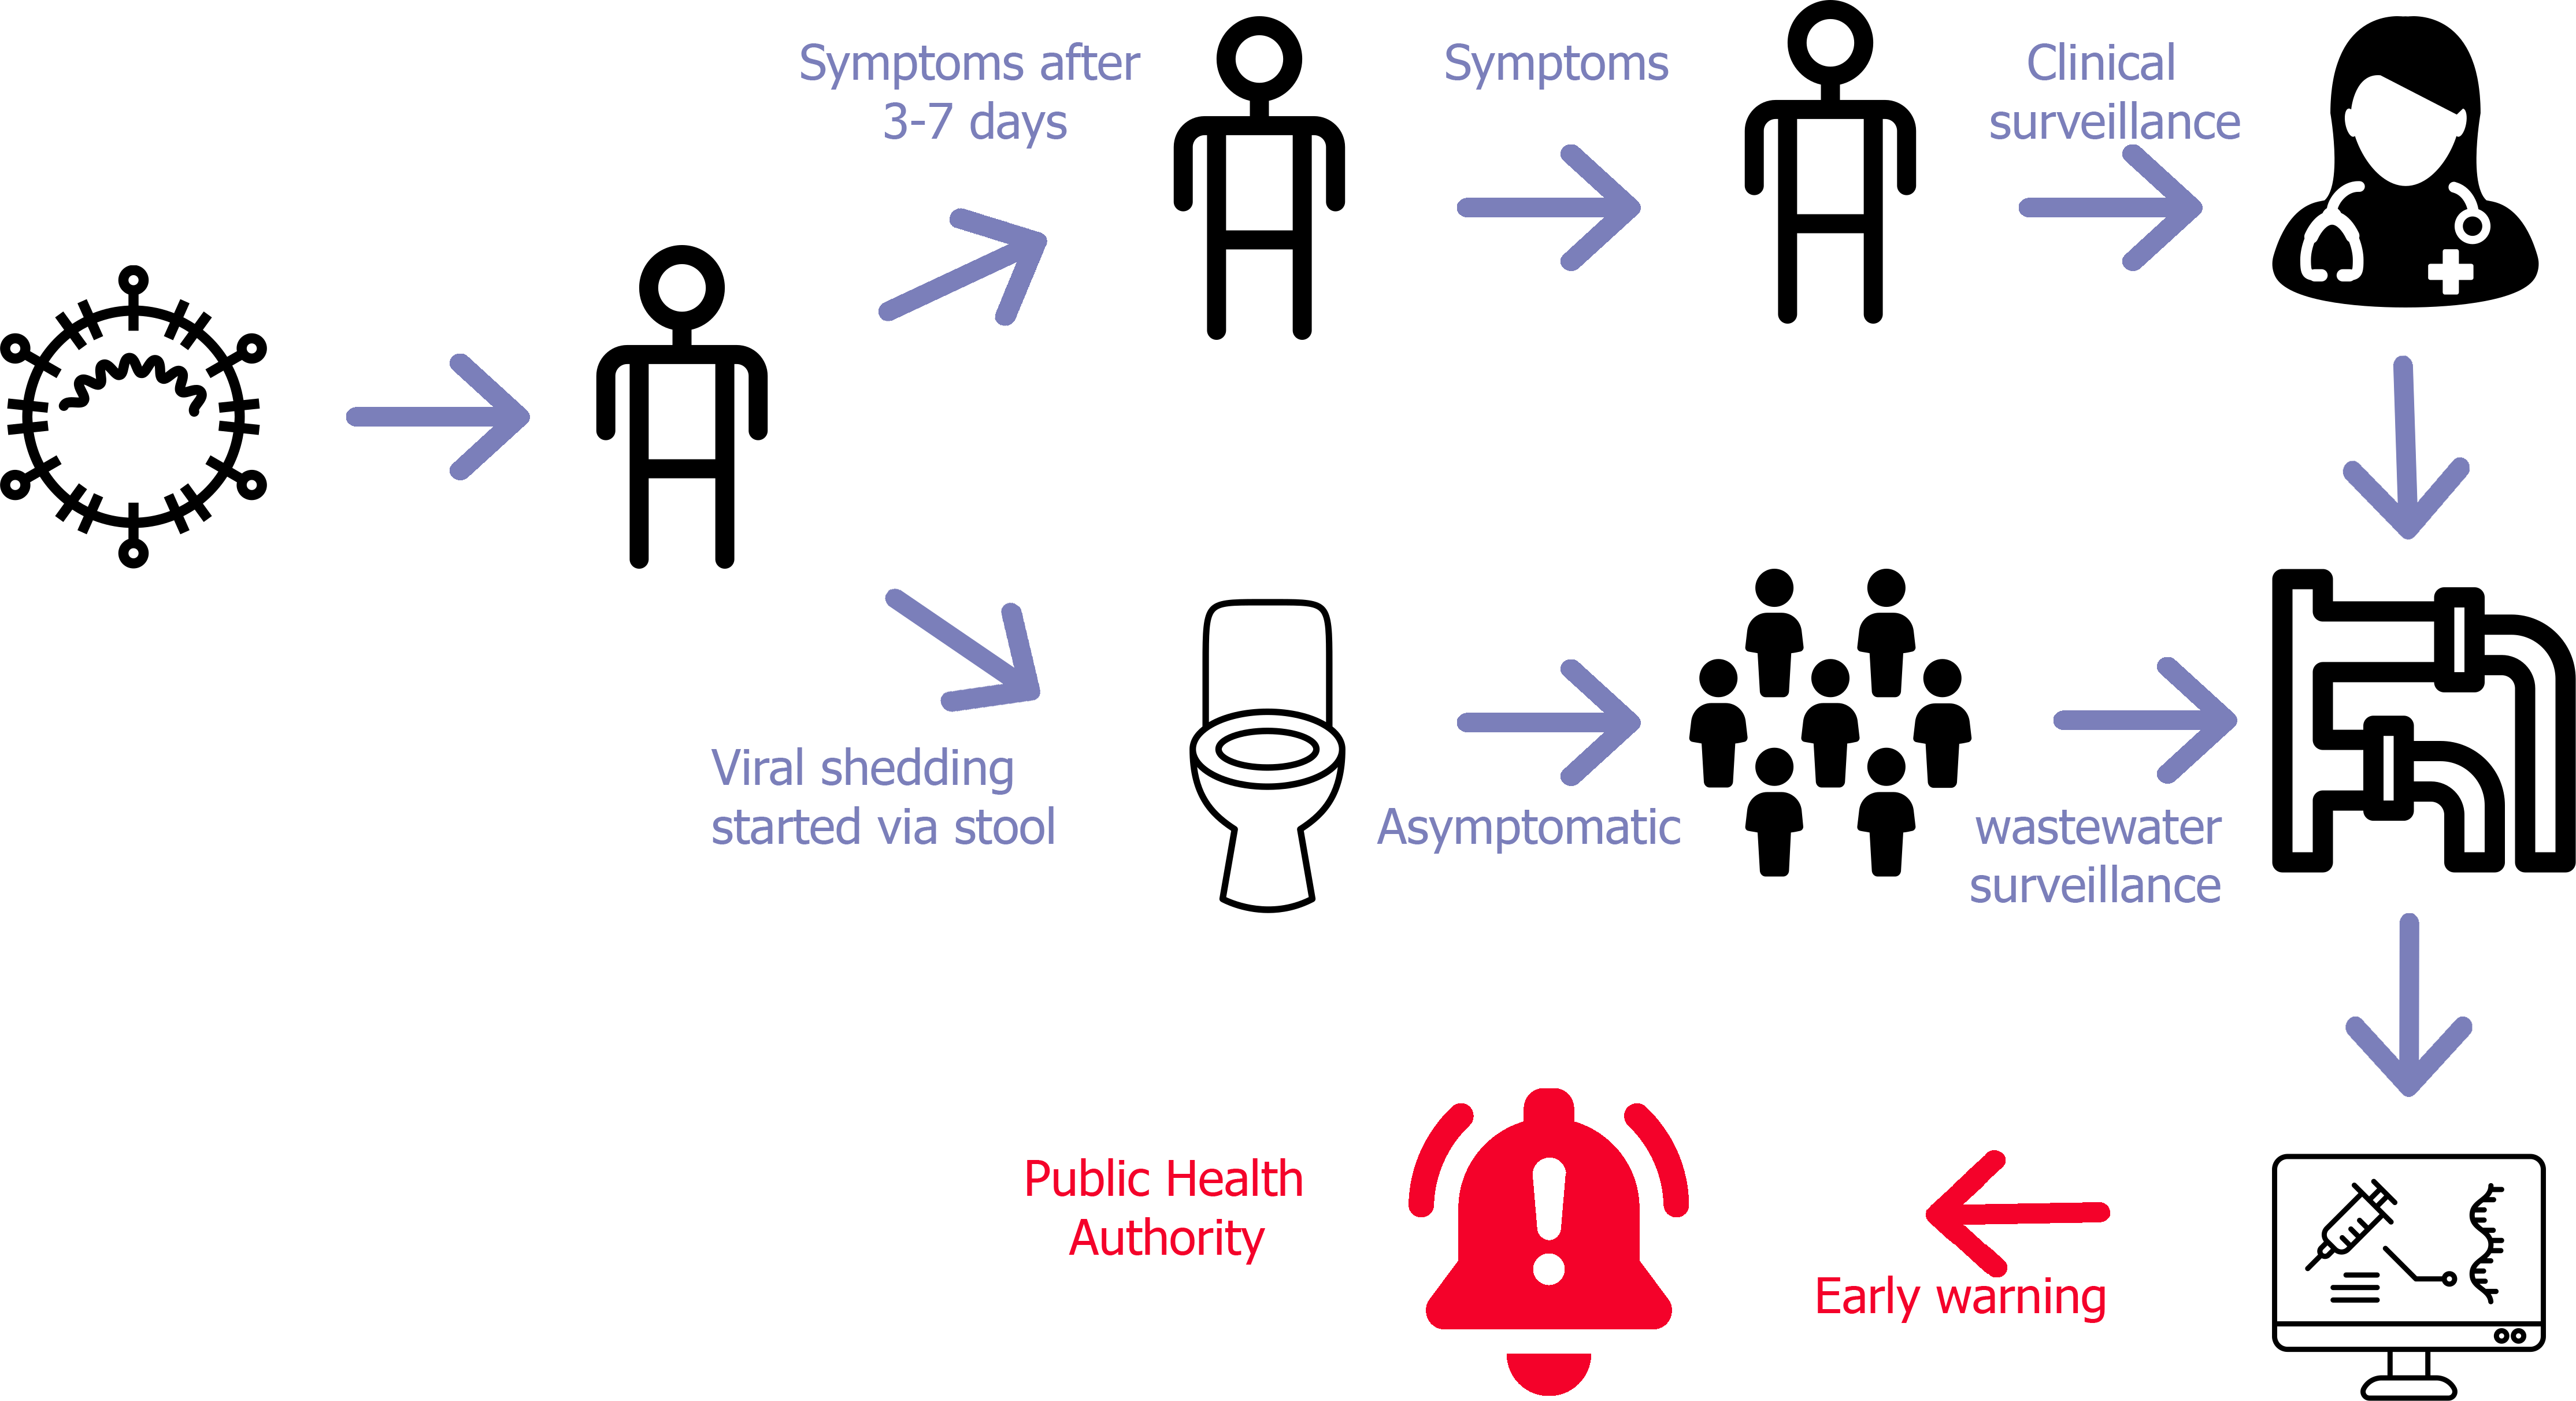
\includegraphics[width=1\textwidth]{figures/intro/ww-process-v2.png}
            \captionof{figure}{Schematic diagram shows the process of detecting viruses by wastewater surveillance against clinical surveillance.}
            \label{fig:intro:ww-process}
        \end{figure}

        \textbf{Where else can wastewater surveillance be used} \\
        
        Viruses are not the only thing that can be monitored in wastewater. This method can be used to detect other microbial pathogens \cite{ko2022}, antimicrobial resistance \cite{hendriksen2019}, or chemical water contaminants \cite{jung2020}. Further, these tools can be used on samples from other settings, such as transport hubs, hospitals, schools, workplaces, and leisure facilities, in addition to wastewater treatment facilities. Besides public-health applications, wastewater surveillance data may be useful to researchers examining community trends and the efficiency of health policies and non-pharmaceutical interventions \cite{wastewater2022}. \\

        \textbf{Wastewater contribution to global safety} \\
        
        Wastewater surveillance provides valuable information on epidemiological developments at the population level that complements case-based surveillance and aids in resource allocation. Likewise, this can be applied to a global scale. Using the wastewater-based epidemiology method, places and communities with poor healthcare accessibility can shed light on the blind spots of pathogen surveillance. A wastewater surveillance system for infectious diseases could contribute to global safety if it is carefully set up and used in a respectful manner.

        The wastewater surveillance methods seem to fit the bill for enabling early, economical, and efficient detection so that public-health measures can be implemented as soon as they are necessary. Globally, wastewater surveillance is poised to become part of public health strategies \cite{hendriksen2019}. \\

        \textbf{SARS-CoV-2 wastewater datasets} \\
        
        Data from wastewater samples should be prepared before they are analyzed. Library preparation refers to this process. To generate SARS-CoV-2 sequence data, several library preparation strategies are used. Therefore, most of these sequencing data are harmonized and available in defined formats from standard repositories, such as ENA in Europe and NCBI SRA in the US \cite{maier2021b}.
        
        As of late May 2022, the ENA sequence read archive contained 13,893 raw samples of SARS-CoV-2 in wastewater datasets (\cref{tab:intro:ww-realdata}). The main statistical numbers are presented in Table. Z. There are the following types of data: 1) Illumina-based Ampliconic; 2) Oxford nanopore (ONT)-based Ampliconic; 3) Illumina-based RNASeq; 4) Oxford nanopore (ONT)-based Whole genome sequencing (WGS); 5) ION-Torrent-based Ampliconic.
        
        \begin{table}[ht!]
            \centering
            \small
            \begin{tabular}{lllll}
            \textbf{Sequencing platform} & \textbf{Library Strategy}        & \textbf{Library Layout}    & \textbf{N of accessions}   & \textbf{N of samples} \\ \hline
            BGISEQ                      & Ampliconic                        & \acrshort{pe}                & 1              & 48 \\
            DNBSEQ                      & Ampliconic                        & \acrshort{pe}                 & 1              & 59 \\
            \acrshort{illumina}         & Ampliconic                    & \acrshort{pe}                   & 21              & 8,100 \\
                                          & RNA-Seq                             & \acrshort{pe}            & 1              & 173 \\
                               & Targeted-Capture                          & \acrshort{pe}            & 1              & 11 \\
                               & \acrshort{wgs}                          & \acrshort{pe}            & 12              & 5,146 \\
            \textbf{\acrshort{illumina} Total}                 &             &           & \textbf{35}              & \textbf{13,430} \\
            ION\_TORRENT                   & Ampliconic & \acrshort{se}             & 4          & 65 \\
            \acrshort{ont}                 & Ampliconic & \acrshort{se}             & 4          & 169\\
                             & \acrshort{wgs} & \acrshort{se}            & 3           & 122\\ 
                              \textbf{\acrshort{ont} Total}                &  &            & \textbf{7}          & \textbf{291}\\\hline
            \textbf{Total}                 &  &             & \textbf{49}           & \textbf{13,893}\\ \hline
            \end{tabular}
            \caption{Overall numbers of accessions and samples of different types of data for SARS-CoV-2 in wastewater datasets in ENA.} \label{tab:intro:ww-realdata}
        \end{table}
        Briefly looking at clinical datasets, one can see similar proportions in late January 2021 for non-wastewater clinical samples. The NCBI sequence read archive contained 190,288 non-wastewater samples \cite{maier2021b} for SARS-CoV-2. The amount of data influenced the further efforts for creating methods to analyze clinical SARS-CoV-2 data, including Galaxy workflows. Illumina-based Ampliconic data remain to be the most commonly obtained for wastewater samples as well as it was for clinical data. \\

        \textbf{Global efforts} \\
        
        Enough efforts have already been made in this direction in the world. Various wastewater tracking projects took place in countries like Estonia \cite{detecting2022,reoveeseire}, Greece \cite{ismart}, and Canada \cite{coalition}. As a result, COVID-19 trends are visualized within the sewer community, contributing to COVID-19 incidence (both reported and unreported). In response to the COVID-19 pandemic, wastewater surveillance data are used to understand and act, and in public health decision-making. COVIDPoops19, a dashboard developed by Colleen Naughton and colleagues at the University of California (UC), Merced, shows monitoring projects for SARS-CoV-2 have sprung up in at least 70 countries since then \cite{naughton2021}. By October 2021, the European Union recommended that all member countries establish monitoring systems for SARS-CoV-2. 26 of 27 countries have adopted this recommendation. In the United States, the National Wastewater Surveillance System includes 400 sites in 19 states. In the U.S., on 2 March 2022, President Joe Biden's administration said the monitoring system would be part of efforts to detect new variants as the Centers for Disease Control and Prevention added a national dashboard of wastewater data. As well, there is a successful project in Bengaluru that has been expanded to half a dozen other cities in India \cite{pandemic2022}. \\

        \textbf{WWS Working Group} \\
        
        At the same time, there are several initiatives to coordinate wastewater surveillance efforts via working groups. For example, 219-nCoV WBE is a Slack space in which worldwide participants share protocols, publications, and other state-of-the-art resources, and help each other. At the European level, a focus group meets every month.
        
    \subsection{Motivation and the goal of the thesis}
    In terms of accessibility and readiness for use, wastewater surveillance pipelines exist with some limitations. Some pipelines demand an upstream set of tools or sub-pipelines that can take some time to prepare datasets. In addition, they are quite strict when it comes to the tools they use. The best performance is achieved by combining different tools in different workflows. Various variant callers were used, for instance, Freebayes in Lineagespot, ShoRAH in V-pipe, and Lofreq in PiGx. Furthermore, the reproducibility of these workflows is not straightforward. Researchers typically receive instructions of varying depths of detail explaining how to launch workflows in their environments. When comes to repeat analysis several times, can turn to some inconveniences. Additionally, researchers are not provided resources to conduct these workflows and downstream analyses afterward. The platform and resources are crucial to research, even though they are a second priority to some scientists.

    In this master thesis, I aim to provide a complete workflow based on Galaxy that provides platforms that can ensure data analysis transparency and reproducibility. To be precise, I intend to adapt the Galaxy workflows developed for clinical data to process wastewater data. In doing so, I integrate existing tools, test these workflows on mock datasets as well as real datasets, and benchmark them against each other and with other solution offered by other researchers.



